\scanpage{47}
% archive foliation: 46
\diagram{\begin{tikzcd}[ampersand replacement=\&,row sep=large]
X_n=\unsure{\widehat{\operatorname{Spec}}|\operatorname{Spec}}\,k[x_n]\arrow[d]\\
X_1=\unsure{\widehat{\operatorname{Spec}}|\operatorname{Spec}}\,k[x_1=z]\arrow[d]\\
X_0=\unsure{\widehat{\operatorname{Spec}}|\operatorname{Spec}}\,k[u]
\end{tikzcd}}
\figure{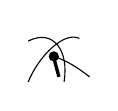
\begin{tikzpicture}[scale=.65]
\draw (-.5,.1) .. controls (0,.35) and (.3,-.1) .. (.2,-.7);
\draw (-.5,-.7) .. controls (-.3,-.2) and (.2,.3) .. (.5,.15);
\draw (0,-.2) .. controls (.3,-.3) and (.5,-.45) .. (.7,-.6);
\fill (0,-.2) circle (.10);\draw[very thick] (0,-.23)--(.1,-.6);
\end{tikzpicture}}
\figure{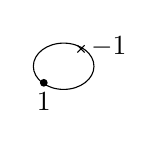
\begin{tikzpicture}[scale=.7]
\draw (0,0) ellipse (.55 and .42);
\fill (-.36,-.30) circle (.07);\node[below] at (-.36,-.30){$1$};
\draw (.25,.38)--(.38,.25) (.25,.25)--(.38,.38);
\node[right] at (.32,.35){$-1$};
\end{tikzpicture}}
\[
\deleted{\unsure{x_n}}\quad x_n^n=x_1
\]
\diagram{\ensuremath{\boxed{\begin{array}{ccc}
n&\left\{\begin{array}{c}1\\1\\\vdots\\1\end{array}\right.&n
\end{array}}}}
\unsure{ramfctn|ramification} au dessus des
$\mathrm{pts}\ 0,\infty$ (où la \unsure{ramfctn|ramification} est $n$)
\unsure{pts} de \unsure{ramfctn|ramification} en haut: $0,\infty$

\diagram{\ensuremath{\boxed{\begin{array}{ccc}2&2&\begin{array}{c}1\\1\end{array}\end{array}}}}
\[
u=\frac12-\frac14(z+z^{-1})
\]
\unsure{ramfctn|ramification} au dessus de

$0$ \deleted{\unsure{pts|pas} \unsure{degrés} (\unsure{pts} au dessus}
\inserted{($z=1$, \unsure{ramfctn|ramification} $2$)}

$1$ ($z=-1$, \unsure{ramfctn|ramification} $2$)

\deleted{\unsure{idem}}

$\infty$ ($0$ et $\infty$ \unsure{ramfctn|ramification} $1$)

\[
\mathbb D_\infty=(\mathbb Z_{/2})\underset{1/2}{\mathord{.}}\mu_\infty
\]
\diagram{\begin{tikzcd}[ampersand replacement=\&,column sep=small,row sep=large]
0\ (n)\arrow[d]\& \&\infty\ (n)\arrow[d]\&1\ (1)\arrow[d,"{\text{\textcircled{\unsure{$n$ fois}}}}"]\&\deleted{\unsure{-1\ (1)}}\arrow[d,draw=none,"{\unsure{\downarrow|-}}" description]\\
0\ (1)\arrow[dr]\&\&\infty\ (1)\arrow[dl]\&1\ (2)\arrow[d,dash]\&-1\ \deleted{\unsure{i\ (n)}}\ (2)\arrow[d]\\
\&\infty\&\&0\&1
\end{tikzcd}}
\margin{$n$ pair}

\figure{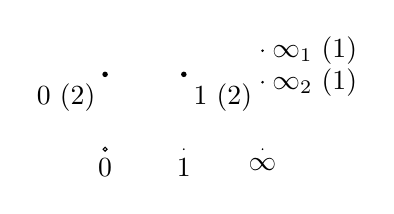
\begin{tikzpicture}
\fill (0,0) circle (.035) node[below left]{$0\ (2)$};
\fill (1,0) circle (.035) node[below right]{$1\ (2)$};
\fill (2,.30) circle (.018) node[right]{$\infty_1\ (1)$};
\fill (2,-.10) circle (.018) node[right]{$\infty_2\ (1)$};
\draw (0,-.95) circle (.025);\node[below] at (0,-.95){$0$};
\fill (1,-.95) circle (.012) node[below]{$1$};
\fill (2,-.95) circle (.012) node[below]{$\infty$};
\end{tikzpicture}}

\figure{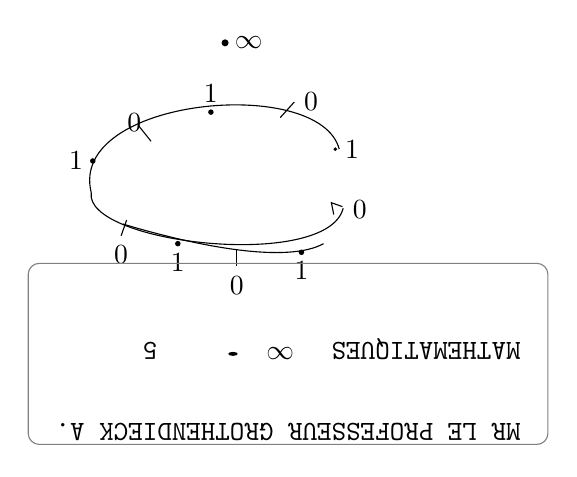
\begin{tikzpicture}[x=1cm,y=1cm]
\fill (0,1.9) circle (.045) node[right]{$\infty$};
\draw (-1.7,0) .. controls (-2,1.2) and (1.2,1.5) .. (1.45,.55);
\draw (-1.7,0) .. controls (-1.8,-.65) and (1.3,-1) .. (1.5,-.2);
\draw (-1.3,-.4) .. controls (-.3,-.7) and (.8,-.9) .. (1.25,-.65);
\fill (-1.68,.4) circle (.035) node[left]{$1$};
\fill (-.18,1.02) circle (.035) node[above]{$1$};
\fill (1.4,.55) circle (.025) node[right]{$1$};
\fill (-.6,-.65) circle (.035) node[below]{$1$};
\fill (.97,-.76) circle (.035) node[below]{$1$};
\draw (-1.1,.85)--(-.94,.65) node[above left]{$0$};
\draw (.7,.95)--(.88,1.15) node[right]{$0$};
\draw (-1.25,-.35)--(-1.32,-.55) node[below]{$0$};
\draw (.15,-.72)--(.15,-.94) node[below]{$0$};
\draw (1.49,-.18)--(1.35,-.13)--(1.38,-.28);\node[right] at (1.5,-.22){$0$};
\draw[gray,rounded corners] (-2.5,-3.2) rectangle (4.1,-.9);
\node[rotate=180,align=left] at (.8,-2.5){\texttt{MR LE PROFESSEUR GROTHENDIECK A.}\\[.6cm]\texttt{MATHEMATIQUES\qquad\qquad\qquad 5}};
\fill (.1,-2.05) ellipse (.06 and .025);\node[right] at (.4,-2.05){$\infty$};
\end{tikzpicture}}
